\section{Logical Database Requirements}

\begin{figure} [H]
    \centering
    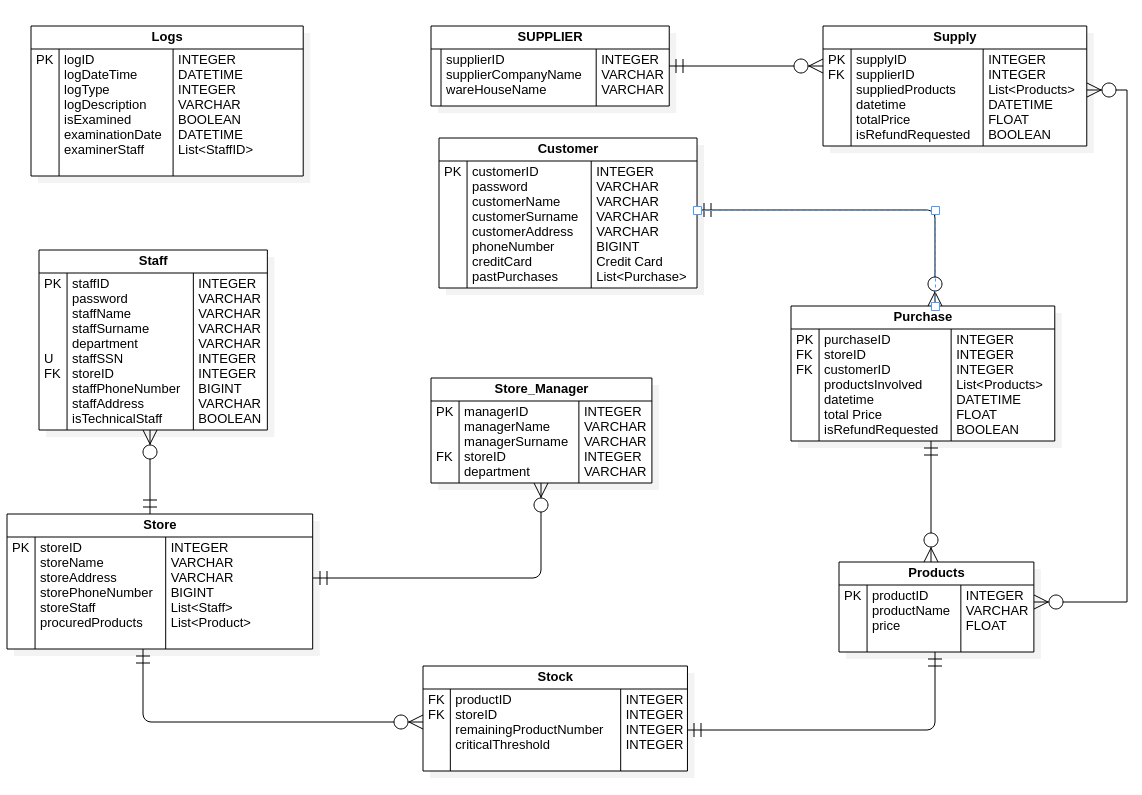
\includegraphics[width=\linewidth]{content/specificRequirements/img/LogicalDatabaseDiagram.png}
    \caption{Logical Database Diagram}
    \label{fig:logical_database_diagram}
\end{figure}


Detailed requirements for the database design and implementation are as follows :
\begin{itemize}
    \item Only store managers shall access to all tables.
    \item Only store managers shall add/remove entries to/from staff table.
    \item Technical staff shall access logs table.
    \item Technical staff shall be capable to add/remove entries to/from logs table. Technical staff shall use technical staff app interface for these kind of operations.
    \item Logs table shall not be accessible except technical staff interface.
    \item Store staff shall access the stock table.
    \item Store staff shall check stocks with store staff interface by accessing this table.
    \item Stock table shall not be accessible except store staff interface.
    \item Only suppliers and store staff groups shall access to the supply table.
    \item Suppliers shall take supply orders by using supplier apps' interface.
    \item Customers shall see and change their own data in the customer table.
    \item Customers shall not see any other customer data.
    \item Customers shall access their private data with the help of customer app interface.
    \item Authorization levels of tables are explained in above detail, other than that, no one shall be able to access a table.
    \item Staffs' password shall be kept encrypted.
    \item Customers' password shall be kept encrypted.
    \item Database backup shall be done every day.
    \item Database backup shall be done in hours which Amazon go store is closed for customers or the most desolated hours of the stores.
    \item Customers table shall have a one-to-many relationship with purchase table since one customer may have more than one purchase with different time, product and store values.
    \item Purchase table shall have a one-to-many relationship with product table since one purchase may have more than one product.
    \item Product table and stock table shall have one-to-one relationship since each product in the store shall have stock value.
    \item Each of the Amazon Go stores shall have more than one stock leads to one-to-many relationship.
    \item Each store shall have manager/s which causes one-to-many relationship.
\end{itemize}
